\documentclass{ximera}
\graphicspath{  %% When looking for images,
{./}            %% look here first,
{./pictures/}   %% then look for a pictures folder,
{../pictures/}  %% which may be a directory up.
{../../pictures/}  %% which may be a directory up.
{../../../pictures/}  %% which may be a directory up.
{../../../../pictures/}  %% which may be a directory up.
}

\usepackage{listings}
%\usepackage{circuitikz}
\usepackage{xcolor}
\usepackage{amsmath,amsthm}
\usepackage{subcaption}
\usepackage{graphicx}
\usepackage{tikz}
%\usepackage{tikz-3dplot}
\usepackage{amsfonts}
%\usepackage{mdframed} % For framing content
%\usepackage{tikz-cd}

  \renewcommand{\vector}[1]{\left\langle #1\right\rangle}
  \newcommand{\arrowvec}[1]{{\overset{\rightharpoonup}{#1}}}
  \newcommand{\ro}{\texttt{R}}%% row operation
  \newcommand{\dotp}{\bullet}%% dot product
  \renewcommand{\l}{\ell}
  \let\defaultAnswerFormat\answerFormatBoxed
  \usetikzlibrary{calc,bending}
  \tikzset{>=stealth}
  




%make a maroon color
\definecolor{maroon}{RGB}{128,0,0}
%make a dark blue color
\definecolor{darkblue}{RGB}{0,0,139}
%define the color fourier0 to be the maroon color
\definecolor{fourier0}{RGB}{128,0,0}
%define the color fourier1 to be the dark blue color
\definecolor{fourier1}{RGB}{0,0,139}
%define the color fourier 1t to be the light blue color
\definecolor{fourier1t}{RGB}{173,216,230}
%define the color fourier2 to be the dark green color
\definecolor{fourier2}{RGB}{0,100,0}
%define teh color fourier2t to be the light green color
\definecolor{fourier2t}{RGB}{144,238,144}
%define the color fourier3 to be the dark purple color
\definecolor{fourier3}{RGB}{128,0,128}
%define the color fourier3t to be the light purple color
\definecolor{fourier3t}{RGB}{221,160,221}
%define the color fourier0t to be the red color
\definecolor{fourier0t}{RGB}{255,0,0}
%define the color fourier4 to be the orange color
\definecolor{fourier4}{RGB}{255,165,0}
%define the color fourier4t to be the darker orange color
\definecolor{fourier4t}{RGB}{255,215,0}
%define the color fourier5 to be the yellow color
\definecolor{fourier5}{RGB}{255,255,0}
%define the color fourier5t to be the darker yellow color
\definecolor{fourier5t}{RGB}{255,255,100}
%define the color fourier6 to be the green color
\definecolor{fourier6}{RGB}{0,128,0}
%define the color fourier6t to be the darker green color
\definecolor{fourier6t}{RGB}{0,255,0}

%New commands for this doc for errors in copying
\newcommand{\eigenvar}{\lambda}
%\newcommand{\vect}[1]{\mathbf{#1}}
\renewcommand{\th}{^{\text{th}}}
\newcommand{\st}{^{\text{st}}}
\newcommand{\nd}{^{\text{nd}}}
\newcommand{\rd}{^{\text{rd}}}
\newcommand{\paren}[1]{\left(#1\right)}
\newcommand{\abs}[1]{\left|#1\right|}
\newcommand{\R}{\mathbb{R}}
\newcommand{\C}{\mathbb{C}}
\newcommand{\Hilb}{\mathbb{H}}
\newcommand{\qq}[1]{\text{#1}}
\newcommand{\Z}{\mathbb{Z}}
\newcommand{\N}{\mathbb{N}}
\newcommand{\q}[1]{\text{``#1''}}
%\newcommand{\mat}[1]{\begin{bmatrix}#1\end{bmatrix}}
\newcommand{\rref}{\text{reduced row echelon form}}
\newcommand{\ef}{\text{echelon form}}
\newcommand{\ohm}{\Omega}
\newcommand{\volt}{\text{V}}
\newcommand{\amp}{\text{A}}
\newcommand{\Seq}{\textbf{Seq}}
\newcommand{\Poly}{\textbf{P}}
\renewcommand{\quad}{\text{    }}
\newcommand{\roweq}{\simeq}
\newcommand{\rowop}{\simeq}
\newcommand{\rowswap}{\leftrightarrow}
\newcommand{\Mat}{\textbf{M}}
\newcommand{\Func}{\textbf{Func}}
\newcommand{\Hw}{\textbf{Hamming weight}}
\newcommand{\Hd}{\textbf{Hamming distance}}
\newcommand{\rank}{\text{rank}}
\newcommand{\longvect}[1]{\overrightarrow{#1}}
% Define the circled command
\newcommand{\circled}[1]{%
  \tikz[baseline=(char.base)]{
    \node[shape=circle,draw,inner sep=2pt,red,fill=red!20,text=black] (char) {#1};}%
}

% Define custom command \strikeh that just puts red text on the 2nd argument
\newcommand{\strikeh}[2]{\textcolor{red}{#2}}

% Define custom command \strikev that just puts red text on the 2nd argument
\newcommand{\strikev}[2]{\textcolor{red}{#2}}

%more new commands for this doc for errors in copying
\newcommand{\SI}{\text{SI}}
\newcommand{\kg}{\text{kg}}
\newcommand{\m}{\text{m}}
\newcommand{\s}{\text{s}}
\newcommand{\norm}[1]{\left\|#1\right\|}
\newcommand{\col}{\text{col}}
\newcommand{\sspan}{\text{span}}
\newcommand{\proj}{\text{proj}}
\newcommand{\set}[1]{\left\{#1\right\}}
\newcommand{\degC}{^\circ\text{C}}
\newcommand{\centroid}[1]{\overline{#1}}
\newcommand{\dotprod}{\boldsymbol{\cdot}}
%\newcommand{\coord}[1]{\begin{bmatrix}#1\end{bmatrix}}
\newcommand{\iprod}[1]{\langle #1 \rangle}
\newcommand{\adjoint}{^{*}}
\newcommand{\conjugate}[1]{\overline{#1}}
\newcommand{\eigenvarA}{\lambda}
\newcommand{\eigenvarB}{\mu}
\newcommand{\orth}{\perp}
\newcommand{\bigbracket}[1]{\left[#1\right]}
\newcommand{\textiff}{\text{ if and only if }}
\newcommand{\adj}{\text{adj}}
\newcommand{\ijth}{\emph{ij}^\text{th}}
\newcommand{\minor}[2]{M_{#2}}
\newcommand{\cofactor}{\text{C}}
\newcommand{\shift}{\textbf{shift}}
\newcommand{\startmat}[1]{
  \left[\begin{array}{#1}
}
\newcommand{\stopmat}{\end{array}\right]}
%a command to give a name to explorations and hints and theorems
\newcommand{\name}[1]{\begin{centering}\textbf{#1}\end{centering}}
\newcommand{\vect}[1]{\vec{#1}}
\newcommand{\dfn}[1]{\textbf{#1}}
\newcommand{\transpose}{\mathsf{T}}
\newcommand{\mtlb}[2][black]{\texttt{\textcolor{#1}{#2}}}
\newcommand{\RR}{\mathbb{R}} % Real numbers
\newcommand{\id}{\text{id}}
\newcommand{\coord}[1]{\langle#1\rangle}
\newcommand{\RREF}{\text{RREF}}
\newcommand{\Null}{\text{Null}}
\newcommand{\Nullity}{\text{Nullity}}
\newcommand{\Rank}{\text{Rank}}
\newcommand{\Col}{\text{Col}}
\newcommand{\Ef}{\text{EF}}
\newcommand{\boxprod}[3]{\abs{(#1\times#2)\cdot#3}}

\author{Zack Reed}
%borrowed from selinger linear algebra
\title{Inner Product Spaces and applications: PCA}
\begin{document}
\begin{abstract}

    One application of IPSs is PCA.

\end{abstract}
\maketitle


\section{Application: Principal component analysis}

%\begin{outcome}
%  \begin{enumerate}
%  \item Compute the principal components of a matrix $A$.
%  \item Compute the centroid of a collection of data points.
%  \item Find the $k$-dimensional subspace that best approximates a
%    given collection of data points.
%  \item Find the $k$-dimensional affine subspace that best
%    approximates a given collection of data points.
%  \item Compute the total squared distance of the data points to the
%    best fit subspace (or best fit affine subspace).
%  \end{enumerate}
%\end{outcome}

In this section, we will explore an application of the diagonalization
of symmetric matrices called \textbf{principal component analysis}.
Imagine we are given a collection of data points such as the
following:
\begin{equation}\label{eqn:subspace-fitting}
  \begin{tikzpicture}[baseline=-0.5ex]
    \draw[thin,->] (-4,0) -- (4,0);
    \draw[thin,->] (0,-4) -- (0,4);
    % \draw[thick,blue] (-4,-4/1.29) -- (4,4/1.29);
    \fill[color=red] (-2.25,-1.21) circle (0.06);
    \fill[color=red] (-1.44,-1.28) circle (0.06);
    \fill[color=red] (2.29,1.82) circle (0.06);
    \fill[color=red] (0.25,0.43) circle (0.06);
    \fill[color=red] (-1.57,-1.07) circle (0.06);
    \fill[color=red] (2.51,2.00) circle (0.06);
    \fill[color=red] (-2.53,-2.34) circle (0.06);
    \fill[color=red] (-3.04,-2.40) circle (0.06);
    \fill[color=red] (0.84,0.36) circle (0.06);
    \fill[color=red] (-3.16,-2.73) circle (0.06);
    \fill[color=red] (-2.02,-1.88) circle (0.06);
    \fill[color=red] (3.06,2.44) circle (0.06);
    \fill[color=red] (-1.40,-1.12) circle (0.06);
    \fill[color=red] (-2.09,-1.34) circle (0.06);
    \fill[color=red] (-1.23,-1.13) circle (0.06);
    \fill[color=red] (0.48,0.06) circle (0.06);
    \fill[color=red] (-1.49,-1.20) circle (0.06);
    \fill[color=red] (0.98,0.75) circle (0.06);
    \fill[color=red] (1.40,0.89) circle (0.06);
    \fill[color=red] (-0.12,0.09) circle (0.06);
    \fill[color=red] (0.88,0.40) circle (0.06);
    \fill[color=red] (-0.38,0.55) circle (0.06);
    \fill[color=red] (0.34,0.46) circle (0.06);
    \fill[color=red] (0.45,0.21) circle (0.06);
    \fill[color=red] (-0.59,-0.63) circle (0.06);
    \fill[color=red] (-0.53,-0.29) circle (0.06);
    \fill[color=red] (2.10,1.35) circle (0.06);
    \fill[color=red] (1.65,1.60) circle (0.06);
    \fill[color=red] (-3.88,-2.83) circle (0.06);
    \fill[color=red] (-0.07,-0.01) circle (0.06);
    \fill[color=red] (-0.37,-0.57) circle (0.06);
    \fill[color=red] (-0.99,-0.75) circle (0.06);
    \fill[color=red] (-2.34,-2.08) circle (0.06);
    \fill[color=red] (3.63,3.15) circle (0.06);
    \fill[color=red] (1.37,0.48) circle (0.06);
    \fill[color=red] (-0.96,-0.74) circle (0.06);
    \fill[color=red] (3.51,2.79) circle (0.06);
    \fill[color=red] (-3.33,-2.72) circle (0.06);
    \fill[color=red] (0.39,0.09) circle (0.06);
    \fill[color=red] (-1.38,-1.17) circle (0.06);
    \fill[color=red] (-0.36,-0.65) circle (0.06);
    \fill[color=red] (1.38,0.66) circle (0.06);
    \fill[color=red] (1.85,1.24) circle (0.06);
    \fill[color=red] (2.35,1.85) circle (0.06);
    \fill[color=red] (0.85,0.25) circle (0.06);
    \fill[color=red] (-0.23,0.19) circle (0.06);
    \fill[color=red] (-0.90,-0.74) circle (0.06);
    \fill[color=red] (2.50,1.31) circle (0.06);
    \fill[color=red] (-0.45,-0.71) circle (0.06);
    \fill[color=red] (0.92,0.56) circle (0.06);
    \fill[color=red] (0.97,1.21) circle (0.06);
    \fill[color=red] (-0.85,-0.74) circle (0.06);
    \fill[color=red] (-0.10,0.13) circle (0.06);
    \fill[color=red] (0.32,0.49) circle (0.06);
    \fill[color=red] (2.58,1.57) circle (0.06);
    \fill[color=red] (-0.59,-0.48) circle (0.06);
    \fill[color=red] (2.28,1.50) circle (0.06);
    \fill[color=red] (1.21,0.94) circle (0.06);
    \fill[color=red] (-0.35,-0.13) circle (0.06);
    \fill[color=red] (-1.53,-1.26) circle (0.06);
    \fill[color=red] (-2.77,-2.14) circle (0.06);
    \fill[color=red] (1.23,1.02) circle (0.06);
    \fill[color=red] (2.61,1.88) circle (0.06);
    \fill[color=red] (-0.04,-0.05) circle (0.06);
    \fill[color=red] (2.09,1.30) circle (0.06);
    \fill[color=red] (2.37,1.52) circle (0.06);
    \fill[color=red] (-2.01,-1.69) circle (0.06);
    \fill[color=red] (0.48,0.72) circle (0.06);
    \fill[color=red] (0.23,0.49) circle (0.06);
    \fill[color=red] (-1.16,-0.95) circle (0.06);
    \fill[color=red] (-0.14,-0.18) circle (0.06);
    \fill[color=red] (-1.57,-1.68) circle (0.06);
    \fill[color=red] (0.39,0.15) circle (0.06);
    \fill[color=red] (-0.24,-0.29) circle (0.06);
  \end{tikzpicture}
\end{equation}
Although these points are spread out in two dimensions, they seem to
be located pretty close to a 1-dimensional subspace. Probably the best
way to interpret this particular data set is to think of the points as
being ``essentially'' on a line, up to some small random errors.

More generally, suppose we are given a collection of data points in
$n$-dimensional space, and we are looking for a $k$-dimensional
subspace that all data points are close to.  This is an important way
to make sense of high-dimensional data. For example, it would be very
difficult to visualize data in a $100$-dimensional space. However, it
we knew that the data points lie very close to a 2-dimensional
subspace, then we could project all of the points to the subspace to
obtain a 2-dimensional image of the data.

To state the problem more precisely, let us introduce the following
notation. If $W$ is a subspace of $\R^n$ and $\vect{v}\in\R^n$ is a
vector, let us write $d(\vect{v},W)$ for the shortest distance from
$\vect{v}$ to $W$ (i.e., the distance from $\vect{v}$ to $W$ along a
line that is perpendicular to $W$). Moreover, if $W$ is a subspace of
$\R^n$ and $\vect{v}_1,\ldots,\vect{v}_m\in\R^n$ are the position
vectors of $m$ points, we define the \textbf{total squared distance}%
\index{distance!total squared distance}%
\index{squared distance}%
\index{total squared distance}%
\index{subspace fitting!total squared distance} of the points to
the subspace to be the quantity
\begin{equation*}
  D = d(\vect{v}_1,W)^2 + \ldots + d(\vect{v}_m,W)^2.
\end{equation*}
Then the problem we would like to solve can be stated as follows:

\begin{problem}{Subspace fitting problem}{subspace-fitting}
  Given vectors $\vect{v}_1,\ldots,\vect{v}_m\in\R^n$ and given an
  integer $k\leq n$, find the $k$-dimensional subspace
  $W\subseteq\R^n$ that minimizes the total squared distance, i.e.,
  such that $D$ is as small as possible%
  \index{subspace fitting}%
  \index{fitting!subspace fitting}.
\end{problem}

The following proposition gives us a method for solving the subspace
fitting problem. It turns out that the key ingredient in solving this
problem is the diagonalization of symmetric matrices. The method was
discovered by Gale Young%
\index{Young, Gale}%
\index{Gale Young} in 1937.

\begin{proposition}{Solution of the subspace fitting problem}{subspace-fitting}
  Given vectors $\vect{v}_1,\ldots,\vect{v}_m\in\R^n$ and $k\leq n$,
  the optimal solution to the subspace fitting problem can be computed
  as follows:
  \begin{enumerate}
  \item Let $A$ be the $m\times n$-matrix whose rows are
    $\vect{v}_1^T,\ldots,\vect{v}_m^T$. (Or equivalently, $A^T$ is the
    $n\times m$-matrix whose columns are
    $\vect{v}_1,\ldots,\vect{v}_m$.)
  \item Let $B=A^TA$. Then $B$ is a positive semidefinite
    $n\times n$-matrix.
  \item By Proposition~\ref{prop:characterize-positive}, all
    eigenvalues of $B$ are real and non-negative. Let
    $\eigenvar_1,\ldots,\eigenvar_n$ be the eigenvalues of $B$, listed
    according to their multiplicity and in decreasing order, i.e., so
    that $\eigenvar_1\geq\eigenvar_2\geq\ldots\geq\eigenvar_n\geq
    0$. Let $\vect{u}_1,\ldots,\vect{u}_n$ be the corresponding
    eigenvectors.
  \item Then $W=\sspan\set{\vect{u}_1,\ldots,\vect{u}_k}$ is the
    solution to the subspace fitting problem.  Moreover, the total
    squared distance of the points to this subspace is
    \begin{equation*}
      D = \eigenvar_{k+1} + \ldots + \eigenvar_n.
    \end{equation*}
  \end{enumerate}
\end{proposition}

\begin{example}{Subspace fitting in $\R^2$}{subspace-fitting-r2}
  Consider the following collection of points in $\R^2$:
  \begin{equation*}
    \set{
      \startmat{r}  2 \\ -3 \stopmat,
      \startmat{r} -1 \\  0 \stopmat,
      \startmat{r}  2 \\  3 \stopmat,
      \startmat{r} -6 \\ -7 \stopmat,
      \startmat{r}  6 \\ 11 \stopmat,
      \startmat{r}  0 \\ -1 \stopmat,
      \startmat{r}  1 \\  6 \stopmat,
      \startmat{r} -2 \\ -3 \stopmat,
      \startmat{r} -7 \\ -6 \stopmat
    }.
  \end{equation*}
  Find the 1-dimensional subspace that best approximates this
  collection of points. What is the total squared distance of the
  points to the subspace?
\end{example}

\begin{solution}
  We follow the steps outlined in
  Proposition~\ref{prop:subspace-fitting}.
  \begin{enumerate}
  \item We have
    \begin{equation*}
      A^T = \startmat{rrrrrrrrr}
        2 & -1 & 2 & -6 & 6 & 0 & 1 & -2 & -7 \\
        -3 & 0 & 3 & -7 & 11 & -1 & 6 & -3 & -6
      \stopmat.
    \end{equation*}
  \item We calculate
    \begin{equation*}
      B = A^TA = \startmat{rr}
        135 & 162 \\
        162 & 270
      \stopmat.
    \end{equation*}
  \item The eigenvalues of $B$ are $\eigenvar_1 = 378$ and
    $\eigenvar_2 = 27$, with corresponding eigenvectors
    \begin{equation*}
      \vect{u}_1 = \startmat{r} 2 \\ 3 \stopmat
      \quad\mbox{and}\quad
      \vect{u}_2 = \startmat{r} 3 \\ -2 \stopmat.
    \end{equation*}
  \item The desired subspace $W$ is spanned by the eigenvector
    corresponding to the largest eigenvalue, i.e.,
    $W=\sspan\set{\vect{u}_1}$. The total squared distance is
    $\eigenvar_2 = 27$.
  \end{enumerate}
  The space $W$ is shown in the following illustration, along with the
  original points:
  \begin{equation*}
    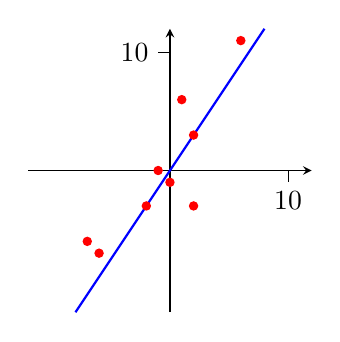
\begin{tikzpicture}[scale=0.15]
      \draw[thin,->] (-12,0) -- (12,0);
      \draw[thin,->] (0,-12) -- (0,12);
      \draw[thin] (0,10) -- (-1,10) node[left] {$10$};
      \draw[thin] (10,0) -- (10,-1) node[below] {$10$};
      \draw[thick,blue] (-8,-12) -- (8,12);
      \fill[color=red] (2,-3) circle (0.4);
      \fill[color=red] (-1, 0) circle (0.4);
      \fill[color=red] (2, 3) circle (0.4);
      \fill[color=red] (-6, -7) circle (0.4);
      \fill[color=red] (6, 11) circle (0.4);
      \fill[color=red] (0, -1) circle (0.4);
      \fill[color=red] (1, 6) circle (0.4);
      \fill[color=red] (-2, -3) circle (0.4);
      \fill[color=red] (-7, -6) circle (0.4);
    \end{tikzpicture}
  \end{equation*}
  Of course, the example was rigged to ensure that the eigenvalues are
  integers. In real life, the entries of $A$ and $B$, as well as the
  eigenvalues and components of the eigenvectors are usually arbitrary
  real numbers.
\end{solution}

\begin{example}{Subspace fitting in $\R^3$}{subspace-fitting-r3}
  Consider the following collection of points in $\R^3$:
  \begin{equation*}
    \set{
      \startmat{r} -7 \\ 4 \\ 5 \stopmat,
      \startmat{r} 0 \\ 3 \\ 3 \stopmat,
      \startmat{r} 2 \\ -5 \\ -4 \stopmat,
      \startmat{r} 10 \\ -4 \\ 1 \stopmat,
      \startmat{r} -2 \\ 5 \\ 4 \stopmat,
      \startmat{r} -8 \\ -1 \\ -5 \stopmat,
      \startmat{r} 5 \\ 4 \\ 2 \stopmat,
      \startmat{r} -6 \\ 9 \\ 6 \stopmat,
      \startmat{r} 9 \\ -6 \\ 3 \stopmat,
      \startmat{r} -2 \\ -7 \\ -8 \stopmat
    }.
  \end{equation*}
  %\begin{enumialphparenastyle}
    \begin{enumerate}
    \item Find the 1-dimensional subspace that best approximates this
      collection of points.
    \item Find the 2-dimensional subspace that best approximates this
      collection of points.
    \item What is the 3-dimensional subspace that best approximates this
      collection of points?
    \end{enumerate}
  %\end{enumialphparenastyle}
  In each case, what is the total squared distance of the points to
  the subspace?
\end{example}

\begin{solution}
  Again, we follow the steps from
  Proposition~\ref{prop:subspace-fitting}. We can do the calculations
  for parts (a), (b), and (c) at the same time.
  \begin{enumerate}
  \item We have
    \begin{equation*}
      A^T = \startmat{rrrrrrrrrr}
        -7 & 0 & 2 & 10 & -2 & -8 & 5 & -6 & 9 & -2 \\
        4 & 3 & -5 & -4 & 5 & -1 & 4 & 9 & -6 & -7 \\
        5 & 3 & -4 & 1 & 4 & -5 & 2 & 6 & 3 & -8 \\
      \stopmat.
    \end{equation*}
  \item We calculate
    \begin{equation*}
      B = A^TA = \startmat{rrr}
        367 & -154 & 16 \\
        -154 & 274 & 170 \\
        16 & 170 & 205 \\
      \stopmat.
    \end{equation*}
  \item The eigenvalues of $B$ are $\eigenvar_1 = 513$,
    $\eigenvar_2 = 306$, and $\eigenvar_3 = 27$, with corresponding
    eigenvectors
    \begin{equation*}
      \vect{u}_1 = \startmat{r} -2 \\ 2 \\ 1 \stopmat,
      \quad
      \vect{u}_2 = \startmat{r} 2 \\ 1 \\ 2 \stopmat
      \quad\mbox{and}\quad
      \vect{u}_3 = \startmat{r} -1 \\ -2 \\ 2 \stopmat.
    \end{equation*}
  \end{enumerate}

  For part (a), the desired 1-dimensional subspace is spanned by the
  eigenvector corresponding to the largest eigenvalue, i.e., it is
  $\sspan\set{\vect{u}_1}$. The total squared distance is
  $\eigenvar_2+\eigenvar_3 = 306 + 27 = 333$.

  For part (b), the desired 2-dimensional subspace is spanned by the
  eigenvectors corresponding to the two largest eigenvalues, i.e., it
  is $\sspan\set{\vect{u}_1,\vect{u}_2}$. The total squared distance is
  $\eigenvar_3 = 27$.

  Finally, in part (c), the desired 3-dimensional subspace is spanned
  by all three eigenvectors; it is of course $\R^3$ itself, since it
  is the only 3-dimensional subspace. The total squared distance is
  $0$, since all points lie in the subspace.
\end{solution}

The vectors $\vect{u}_1,\ldots,\vect{u}_n$ that appear in the solution
of the subspace fitting problem are called the \textbf{principal
  components} of the matrix $A$.

\begin{definition}{Principal components}{principal-components}
  Let $A$ be an $m\times n$-matrix. The \textbf{principal components}%
  \index{principal component}%
  \index{component!principal component} of $A$ are the (normalized,
  orthogonal) eigenvectors $\vect{u}_1,\ldots,\vect{u}_n$ of the
  positive semidefinite $n\times n$-matrix $A^TA$. They are usually
  listed in order of decreasing eigenvalues.
\end{definition}

The first principal component $\vect{u}_1$ gives the direction in
which the rows of $A$ show the most variability. The second principal
component $\vect{u}_2$ gives the direction in which the rows of $A$
show the most remaining variability that is orthogonal to
$\vect{u}_1$. The third principal component $\vect{u}_3$ gives the
direction of most variability that is orthogonal to $\vect{u}_1$ and
$\vect{u}_2$, and so on.

% ----------------------------------------------------------------------
\subsection*{Subspace fitting vs. curve fitting}

In the particular case where $n=2$ and $k=1$, we are looking for a
1-dimensional subspace, i.e., a line through the origin, which best
fits the given 2-dimensional data, as in the illustration
{\eqref{eqn:subspace-fitting}} above or as in
Example~\ref{exa:subspace-fitting-r2}. On its face, the subspace
fitting problem in this case seems similar to the linear curve
fitting%
\index{curve fitting} problem we solved in
Section~\ref{sec:least-squares}. However, there is a subtle but
important difference: in linear curve fitting, we were seeking to
minimize the distances of the points from the line in the
$y$-direction, whereas in subspace fitting, we are seeking to minimize
the distances of the points from the subspace in the direction
perpendicular to the subspace. The following pair of pictures
illustrates the difference:
\begin{equation*}
  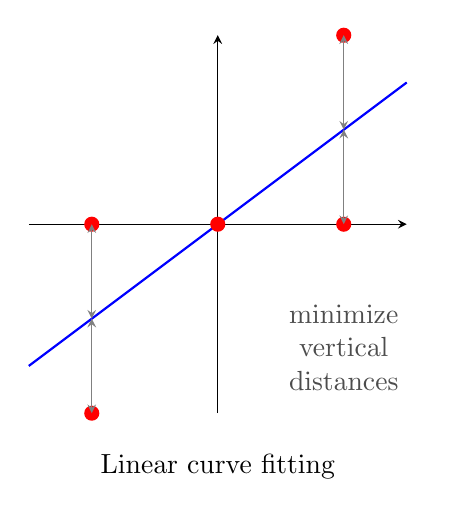
\begin{tikzpicture}[scale=0.8]
    \draw[thin,->] (-3,0) -- (3,0);
    \draw[thin,->] (0,-3) -- (0,3);
    \draw[thick,blue] (-3,-3*0.75) -- (3,3*0.75);
    \fill[color=red] (0,0) circle (0.12);
    \fill[color=red] (2,0) circle (0.12);
    \fill[color=red] (2,3) circle (0.12);
    \fill[color=red] (-2,0) circle (0.12);
    \fill[color=red] (-2,-3) circle (0.12);
    \draw[<->,black!50] (2,0) -- (2,1.5);
    \draw[<->,black!50] (2,3) -- (2,1.5);
    \draw[<->,black!50] (-2,0) -- (-2,-1.5);
    \draw[<->,black!50] (-2,-3) -- (-2,-1.5);
    \path (0,-3.5) node[below] {Linear curve fitting};
    \path[black!70] (2,-2) node {\begin{tabular}{c}minimize\\vertical\\distances\end{tabular}};
  \end{tikzpicture}
  \hspace{1in}
  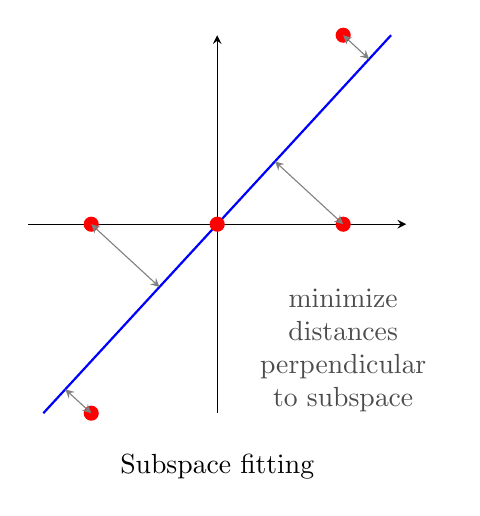
\begin{tikzpicture}[scale=0.8]
    \draw[thin,->] (-3,0) -- (3,0);
    \draw[thin,->] (0,-3) -- (0,3);
    \draw[thick,blue] (-3*0.92,-3) -- (3*0.92, 3);
    \fill[color=red] (0,0) circle (0.12);
    \fill[color=red] (2,0) circle (0.12);
    \fill[color=red] (2,3) circle (0.12);
    \fill[color=red] (-2,0) circle (0.12);
    \fill[color=red] (-2,-3) circle (0.12);
    \draw[<->,black!50] (2,0) -- (0.997*0.92,0.997);
    \draw[<->,black!50] (2,3) -- (2.621*0.92,2.621);
    \draw[<->,black!50] (-2,0) -- (-0.997*0.92,-0.997);
    \draw[<->,black!50] (-2,-3) -- (-2.621*0.92,-2.621);
    \path (0,-3.5) node[below] {Subspace fitting};
    \path[black!70] (2,-2) node {\begin{tabular}{c}minimize\\distances\\perpendicular\\to subspace\end{tabular}};
  \end{tikzpicture}
\end{equation*}

% ----------------------------------------------------------------------
\subsection*{Affine fitting}

So far, we have been looking to approximate a given collection of
points by a {\em subspace}, which necessarily passes through the
origin. But sometimes the points may not be near the origin, as in
this example:
\begin{equation*}
  \begin{tikzpicture}[baseline=-0.5ex, scale=0.8]
    \draw[thin,->] (-4,0) -- (4,0);
    \draw[thin,->] (0,-4) -- (0,4);
    % \draw[thick, blue] (0.91,1.76) +(-6,-6/-3.20) -- +(6,6/-3.20);
    \fill[color=red] (-0.54,2.53) circle (0.075);
    \fill[color=red] (4.26,0.53) circle (0.075);
    \fill[color=red] (-0.24,2.38) circle (0.075);
    \fill[color=red] (1.98,1.52) circle (0.075);
    \fill[color=red] (0.28,2.14) circle (0.075);
    \fill[color=red] (5.71,0.05) circle (0.075);
    \fill[color=red] (2.90,1.56) circle (0.075);
    \fill[color=red] (-3.21,2.97) circle (0.075);
    \fill[color=red] (5.44,-0.09) circle (0.075);
    \fill[color=red] (-0.37,1.87) circle (0.075);
    \fill[color=red] (-0.46,2.02) circle (0.075);
    \fill[color=red] (2.21,1.49) circle (0.075);
    \fill[color=red] (-0.91,2.23) circle (0.075);
    \fill[color=red] (0.81,1.80) circle (0.075);
    \fill[color=red] (0.47,1.91) circle (0.075);
    \fill[color=red] (0.96,2.34) circle (0.075);
    \fill[color=red] (-0.93,2.29) circle (0.075);
    \fill[color=red] (-0.35,2.09) circle (0.075);
    \fill[color=red] (1.99,1.11) circle (0.075);
    \fill[color=red] (2.34,1.31) circle (0.075);
    \fill[color=red] (-0.99,2.30) circle (0.075);
    \fill[color=red] (-2.26,2.78) circle (0.075);
    \fill[color=red] (4.07,0.84) circle (0.075);
    \fill[color=red] (0.50,2.19) circle (0.075);
    \fill[color=red] (-1.08,2.76) circle (0.075);
    \fill[color=red] (-0.10,2.07) circle (0.075);
    \fill[color=red] (1.49,1.46) circle (0.075);
    \fill[color=red] (2.05,1.08) circle (0.075);
    \fill[color=red] (4.18,0.74) circle (0.075);
    \fill[color=red] (0.29,1.98) circle (0.075);
    \fill[color=red] (-1.37,2.64) circle (0.075);
    \fill[color=red] (0.75,2.22) circle (0.075);
    \fill[color=red] (0.55,1.91) circle (0.075);
    \fill[color=red] (2.41,1.73) circle (0.075);
    \fill[color=red] (3.70,1.02) circle (0.075);
    \fill[color=red] (1.73,1.85) circle (0.075);
    \fill[color=red] (-0.03,1.99) circle (0.075);
    \fill[color=red] (2.60,1.00) circle (0.075);
    \fill[color=red] (-0.57,2.42) circle (0.075);
    \fill[color=red] (2.44,0.87) circle (0.075);
    \fill[color=red] (1.67,1.20) circle (0.075);
    \fill[color=red] (2.27,1.53) circle (0.075);
    \fill[color=red] (-1.48,2.27) circle (0.075);
    \fill[color=red] (-0.65,1.73) circle (0.075);
    \fill[color=red] (3.53,0.83) circle (0.075);
    \fill[color=red] (0.00,2.10) circle (0.075);
    \fill[color=red] (0.03,2.06) circle (0.075);
    \fill[color=red] (-0.40,2.34) circle (0.075);
    \fill[color=red] (0.48,1.91) circle (0.075);
    \fill[color=red] (-0.59,2.74) circle (0.075);
    \fill[color=red] (0.71,1.61) circle (0.075);
    \fill[color=red] (-0.04,1.88) circle (0.075);
    \fill[color=red] (0.33,1.89) circle (0.075);
    \fill[color=red] (4.66,0.67) circle (0.075);
    \fill[color=red] (3.68,1.23) circle (0.075);
    \fill[color=red] (1.06,1.51) circle (0.075);
    \fill[color=red] (-0.08,2.08) circle (0.075);
    \fill[color=red] (-0.24,1.75) circle (0.075);
    \fill[color=red] (4.36,0.91) circle (0.075);
    \fill[color=red] (1.17,1.51) circle (0.075);
    \fill[color=red] (1.25,2.07) circle (0.075);
    \fill[color=red] (2.36,1.48) circle (0.075);
    \fill[color=red] (-1.21,2.26) circle (0.075);
    \fill[color=red] (-0.13,1.83) circle (0.075);
    \fill[color=red] (1.23,1.51) circle (0.075);
    \fill[color=red] (2.30,1.40) circle (0.075);
    \fill[color=red] (-1.08,2.50) circle (0.075);
    \fill[color=red] (-1.62,2.33) circle (0.075);
    \fill[color=red] (-0.27,2.32) circle (0.075);
    \fill[color=red] (-1.75,2.52) circle (0.075);
    \fill[color=red] (3.37,1.10) circle (0.075);
    \fill[color=red] (-1.10,2.10) circle (0.075);
    \fill[color=red] (-0.54,1.85) circle (0.075);
    \fill[color=red] (2.16,1.16) circle (0.075);
    \fill[color=red] (-0.15,2.11) circle (0.075);
  \end{tikzpicture}
\end{equation*}
In this case, approximating the points by a subspace passing through
the origin does not make much sense. Instead, we should be looking for
an \textbf{affine subspace}. An affine subspace is similar to a
subspace, except it does not necessarily contain the origin.

\begin{definition}{Affine subspace}{affine-subspace}
  Let $V$ be a vector space. A subset $A\subseteq V$ is called an
  \textbf{affine subspace}%
  \index{affine subspace}%
  \index{subspace!affine} of $V$ if $A$ is either empty, or else of
  the form
  \begin{equation*}
    A = \vect{v} + W = \set{\vect{v}+\vect{w} \mid \vect{w}\in W},
  \end{equation*}
  where $\vect{v}\in V$ and $W$ is a subspace of\/ $V$.
\end{definition}

For example, in Chapter~\ref{cha:lines-and-planes}, we considered
lines and planes in $\R^n$ that pass through a given point (not
necessarily the origin). These are examples of affine subspaces of
$\R^n$. The affine subspace fitting problem is analogous to the
subspace fitting problem:

\begin{problem}{Affine subspace fitting problem}{affine-subspace-fitting}
  Given the position vectors $\vect{v}_1,\ldots,\vect{v}_m$ of $m$
  points in $\R^n$, and given an integer $k\leq n$, find the
  $k$-dimensional affine subspace $A\subseteq\R^n$ that minimizes the
  total squared distance from the points to $A$%
  \index{affine subspace fitting}%
  \index{subspace fitting!affine}%
  \index{fitting!affine subspace fitting}.
\end{problem}

It turns out that the optimal solution to the affine subspace fitting
problem can be computed by first computing the \textbf{centroid} of
the points, shifting the whole problem so that the centroid is at the
origin, and then solving an ordinary subspace fitting problem.

\begin{definition}{Centroid}{centroid}
  Given $m$ vectors $\vect{v}_1,\ldots,\vect{v}_m$, their
  \textbf{centroid}%
  \index{centroid} is the vector
  \begin{equation*}
    \centroid{\vect{v}} = \frac{1}{m}(\vect{v}_1+\ldots+\vect{v}_m).
  \end{equation*}
  It is also sometimes called the \textbf{average}%
  \index{average!of vectors} or the \textbf{center of mass}%
  \index{center of mass} of the vectors.
\end{definition}

\begin{proposition}{Solution of the affine subspace fitting problem}{affine-subspace-fitting}
  Given vectors $\vect{v}_1,\ldots,\vect{v}_m\in\R^n$ and $k\leq n$,
  the optimal solution to the affine subspace fitting problem can be
  computed as follows:
  \begin{enumerate}
  \item Compute the centroid $\centroid{\vect{v}} =
    \frac{1}{m}(\vect{v}_1+\ldots+\vect{v}_m)$ of the vectors.
  \item Let $\vect{w}_i = \vect{v}_i - \centroid{\vect{v}}$, for all
    $i=1,\ldots,n$.
  \item Compute the solution $W$ to the (ordinary) subspace fitting
    problem for $\vect{w}_1,\ldots,\vect{w}_m$, as in
    Proposition~\ref{prop:subspace-fitting}.
  \end{enumerate}
  Then the best solution to the affine subspace problem is
  $\centroid{\vect{v}} + W$.
\end{proposition}

\begin{example}{Affine subspace fitting problem}{affine-subspace-fitting}
  Consider the following collection of points in $\R^2$:
  \begin{equation*}
    \set{
      \startmat{r} 10 \\ -6 \stopmat,
      \startmat{r} 2 \\ 10 \stopmat,
      \startmat{r} 5 \\ -1 \stopmat,
      \startmat{r} 8 \\ 3 \stopmat,
      \startmat{r} 2 \\ 5 \stopmat,
      \startmat{r} 3 \\ 3 \stopmat,
      \startmat{r} 4 \\ 11 \stopmat,
      \startmat{r} 10 \\ -1 \stopmat,
      \startmat{r} 1 \\ 12 \stopmat
    }.
  \end{equation*}
  Find the 1-dimensional affine subspace that best approximates this
  collection of points. What is the total squared distance of the
  points to the subspace?
\end{example}

\begin{solution}
  We start by computing the centroid:
  \begin{equation*}
    \centroid{\vect{v}} =
    \frac{1}{9}(\vect{v}_1+\ldots+\vect{v}_9)
    = \frac{1}{9}\startmat{r} 45 \\ 36 \stopmat
    = \startmat{r} 5 \\ 4 \stopmat.
  \end{equation*}
  Next, we shift all vectors by $-\centroid{\vect{v}}$ to get a new
  collection of vectors $\vect{w}_1,\ldots,\vect{w}_9$ centered at the
  origin.
  For example,
  \begin{eqnarray*}
    \vect{w}_1 ~~=~~ \vect{v}_1 - \centroid{\vect{v}}
    &=& \startmat{r} 10 \\ -6 \stopmat
    - \startmat{r} 5 \\ 4 \stopmat
    ~~=~~ \startmat{r} 5 \\ -10 \stopmat,
    \\
    \vect{w}_2 ~~=~~ \vect{v}_2 - \centroid{\vect{v}}
    &=& \startmat{r} 2 \\ 10 \stopmat
    - \startmat{r} 5 \\ 4 \stopmat
    ~~=~~ \startmat{r} -3 \\ 6 \stopmat,
  \end{eqnarray*}
  and so on. We get
  \begin{equation*}
    \set{\vect{w}_1,\ldots,\vect{w}_9} =
    \set{
      \startmat{r} 5 \\ -10 \stopmat,
      \startmat{r} -3 \\ 6 \stopmat,
      \startmat{r} 0 \\ -5 \stopmat,
      \startmat{r} 3 \\ -1 \stopmat,
      \startmat{r} -3 \\ 1 \stopmat,
      \startmat{r} -2 \\ -1 \stopmat,
      \startmat{r} -1 \\ 7 \stopmat,
      \startmat{r} 5 \\ -5 \stopmat,
      \startmat{r} -4 \\ 8 \stopmat
    }.
  \end{equation*}
  Next we, we proceed as in Proposition~\ref{prop:subspace-fitting} to
  find the best subspace fitting $\vect{w}_1,\ldots,\vect{w}_9$. We
  have
  \begin{equation*}
    A^T = \startmat{rrrrrrrrr}
      5 & -3 & 0 & 3 & -3 & -2 & -1 & 5 & -4 \\
      -10 & 6 & -5 & -1 & 1 & -1 & 7 & -5 & 8 \\
    \stopmat
  \end{equation*}
  and
  \begin{equation*}
    B = A^TA = \startmat{rr}
      98 & -136 \\
      -136 & 302 \\
    \stopmat.
  \end{equation*}
  The eigenvalues of $B$ are $\eigenvar_1 = 370$ and $\eigenvar_2 =
  30$, with corresponding eigenvectors
  \begin{equation*}
    \vect{u}_1 = \startmat{r} 1 \\ -2 \stopmat
    \quad\mbox{and}\quad
    \vect{u}_2 = \startmat{r} 2 \\ 1 \stopmat
  \end{equation*}
  Thus, the best-fitting 1-dimensional subspace for
  $\vect{w}_1,\ldots,\vect{w}_9$ is $W = \sspan\set{\vect{u}_1}$, and
  the best-fitting 1-dimensional affine subspace for
  $\vect{v}_1,\ldots,\vect{v}_9$ is
  \begin{equation*}
    \centroid{\vect{v}} + W
    = \set{\centroid{\vect{v}} + \vect{w} \mid \vect{w}\in W}
    = \set{\left.\startmat{r} 5 \\ 4 \stopmat +
        t\startmat{r} 1 \\ -2 \stopmat ~\right\vert~ t\in\R}.
  \end{equation*}
  Note that this is the equation of a line passing through the
  centroid $\centroid{\vect{v}}$, and with direction vector
  $\vect{u}_1$. The points $\vect{v}_1,\ldots,\vect{v}_9$, their
  centroid, and the affine subspace $\centroid{\vect{v}} + W$ are
  shown in the following illustration:
  \begin{equation*}
    \begin{tikzpicture}[scale=0.2]
      \draw[thin,->] (-12,0) -- (12,0);
      \draw[thin,->] (0,-12) -- (0,12);
      \draw[thin] (0,10) -- (-1,10) node[left] {$10$};
      \draw[thin] (10,0) -- (10,-1) node[below] {$10$};
      \draw[thick,blue] (5,4) +(-6,12) -- +(6,-12);
      \fill[color=blue] (5,4) circle (0.6);
      \draw[blue, ->] (5,4) +(8,4) node[right,yshift=4] {centroid} -- +(0.4,0.2);
      \fill[color=red] (10, -6) circle (0.3);
      \fill[color=red] (10, -1) circle (0.3);
      \fill[color=red] (5, -1) circle (0.3);
      \fill[color=red] (8, 3) circle (0.3);
      \fill[color=red] (3, 3) circle (0.3);
      \fill[color=red] (2, 5) circle (0.3);
      \fill[color=red] (2, 10) circle (0.3);
      \fill[color=red] (4, 11) circle (0.3);
      \fill[color=red] (1, 12) circle (0.3);
    \end{tikzpicture}
  \end{equation*}
  \vspace{-4ex}\par  
\end{solution}


\end{document}